\documentclass[paper.tex]{subfiles}

\begin{document}

\section{Introduction and background}

This report is heavily based on Robert Ghrist's \emph{An ODE whose solutions contain all knots and links}~\cite{knottyode}. In that manuscript, Ghrist gives an excellent high-level exposition of a proof that an ODE containing
all knots and links as periodic orbits exists, building heavily off of his existing work in this area. His manuscript is chock full of interesting side notes; the connection between knot theory and dynamical systems is so rich
that it's difficult to not get distracted by the

Rather than pointlessly recapitulate what Ghrist has already stated so elegantly, we seek to give a more compact and self-contained exposition of the beautiful proof that the required ODE exists. The reader is encouraged to
refer to Ghrist's review papers \cite{knottyode}\cite{chaoticknots}to see many many interesting footnotes and connections that will not make it into this work.

We will inevitably be unable to resist the temptation to discuss at least a few interesting connections and questions. The last section of this manuscript is reserved for discussion of those distractions that most fascinate the
authors during the writing.

As briefly stated above, our ultimate goal is to prove the existence of a universal ODE, an ODE whose periodic solutions contain all knots and links.


\subsection{Templates}

The story begins with \emph{templates}, a beautiful and very powerful construction. It would be very difficult to prove the existence of a universal ODE working directly with ODEs, so following one of the main mantras
of mathematics, we collapse out things that are the `same' and obtain a new object. In this case, we collapse out along the stable direction of a given ODE, identifying all orbits which share the same asymptotic future.
This transforms a flow on a three-dimensional manifold into a flow to a semiflow (a one directional flow) on a branched two-dimensional manifold.

We do not discuss the intricacies of this construction, for details, see~\cite{bw1983b}.


\begin{definition}[Template]
  A \emph{template} is a compact branched two-manifold fitted with a smooth expansive semiflow and built from a finite number of \emph{joining} and \emph{splitting} charts, as in Figure~\ref{fig:joinsplit}~\cite{knottyode}.
\end{definition}


\begin{figure}[h]
  \centering
  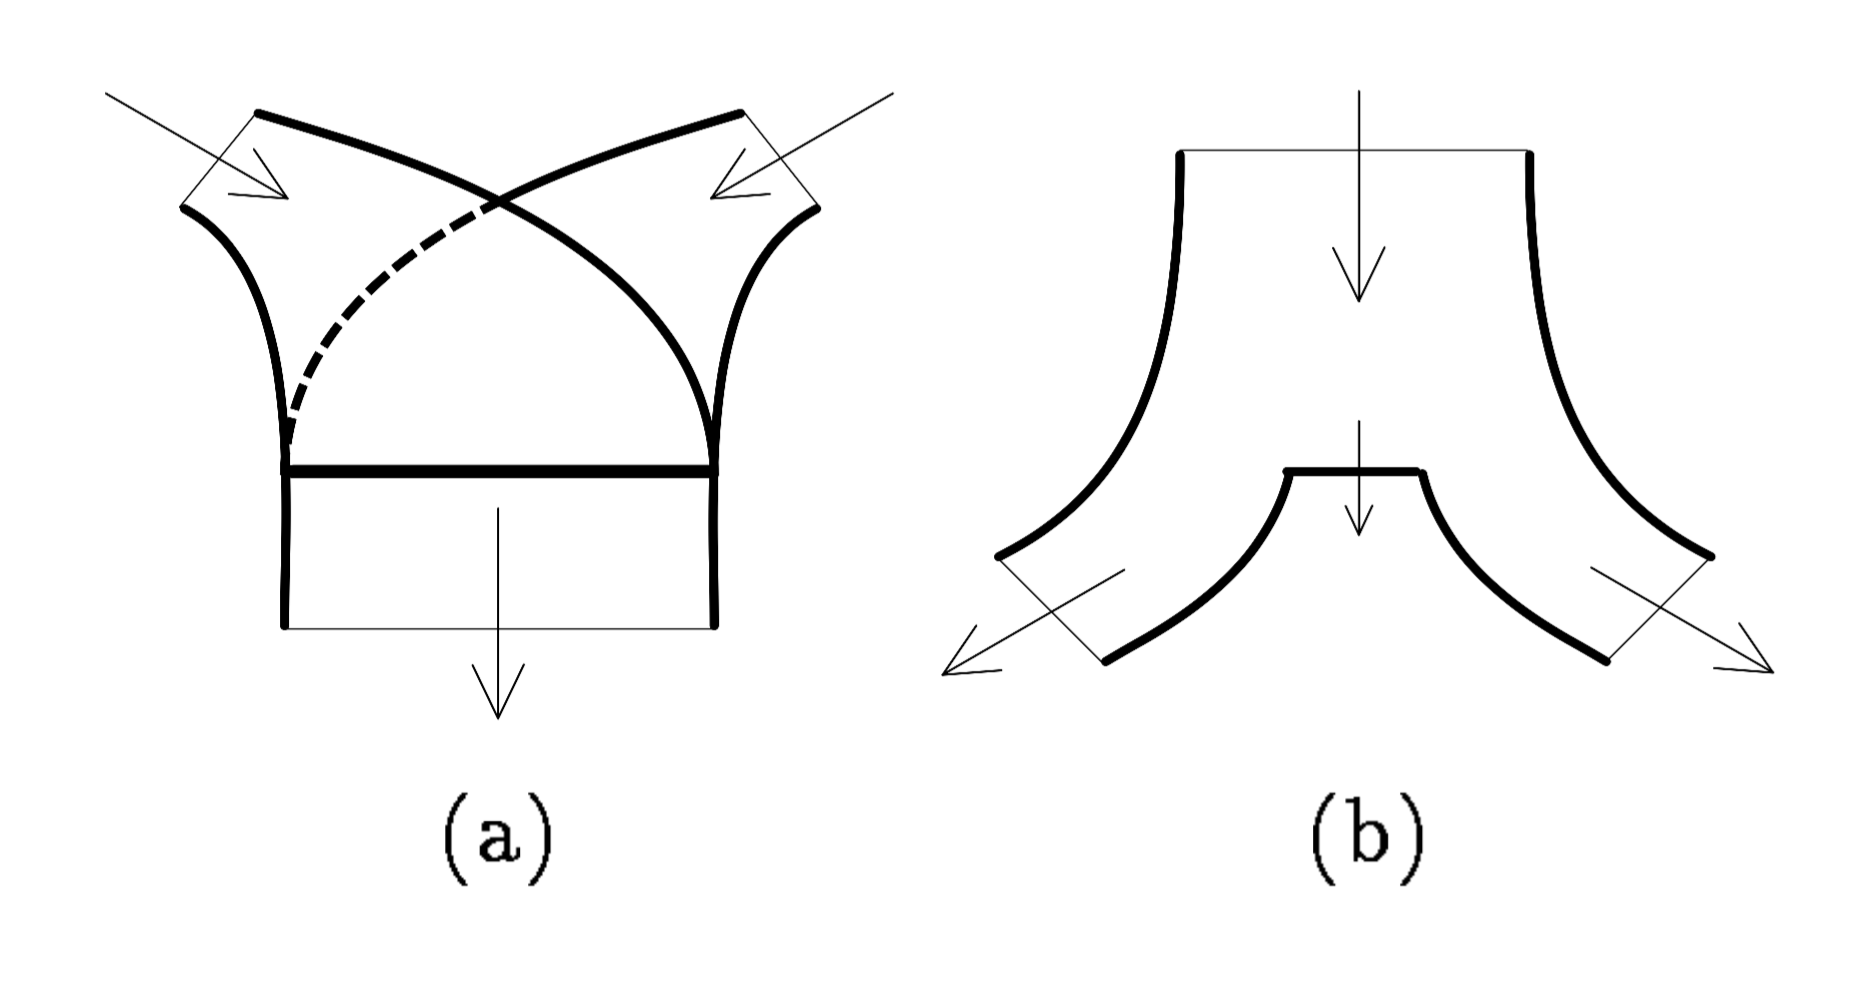
\includegraphics[width=0.5\textwidth]{joining_splitting.png}
  \caption[what goes here]{(a) joining and (b) splitting charts, reproduced from~\cite{knottyode}\protect\footnotemark}\label{fig:joinsplit}
\end{figure}

% how to get this to display?
\footnotetext{Regrettably, without permission}

\begin{figure}[h]
  \centering
  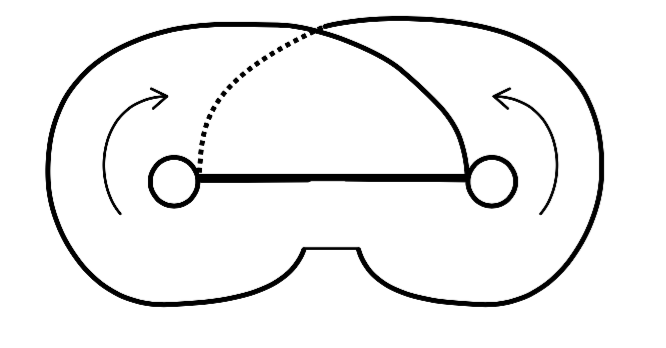
\includegraphics[width=0.5\textwidth]{lorenz.png}
  \caption{The Lorenz template, reproduced from~\cite{knottyode}}\label{fig:lorenz}
\end{figure}

Figure~\ref{fig:lorenz} shows the template for the familiar Lorenz system, the canonical chaotic system, described in equation~\ref{eq:lorenz}. The simplicity of the Lorenz template is a testament to the elegance of
templates - the Lorenz template exactly captures the repeated expanding and folding over of orbits that is the signature of chaos. For certain parameter values, periodic solutions to these equations form a link of infinitely
many components, although we will see later that the Lorenz system is not universal.

\begin{align*}
  \label{eq:lorenz}
  \dot{x} &= \sigma(y - x ) \\
  \dot{y} &= \beta x - y - x z \\
  \dot{z} &= - \beta z + x y
\end{align*}

The primary formal advantage of working with templates, is that they allow the use of \emph{symbolic dynamics}. We can identify periodic orbits on a template $\tau$ with the sequence of strips crossed.

\begin{definition}
  Following~\cite{knottyode}, given a template $\tau$, we define
  \begin{itemize}
    \item Branch lines  $\set{l_j : j = 1, \cdots M}$, the one-dimensional lines strips are connected along
    \item Strips $\set{x_i : i = 1, \cdots N \geq 2 M}$, the two-dimensional regions connecting branch lines
    \item Itinerary $(x_{s_1}x_{s_2}x_{s_3} \dots)$, a sequence of strips crossed by an orbit on $\tau$
    \item Itinerary space $\Sigma_\tau = \set{a_0 a_1 a_2 \cdots} \subset \set{x_1, x_2, \ldots, x_N}^{\Z^+}$, the set of all possible itineraries on $\tau$
    \item Transition matrix

      \begin{equation}
        A_\tau(i,j) = \left\{ \
        \begin{smallmatrix}
          0 \text{ if } \not\exists \text{ a strip from } x_i \text{ to } x_j \\
          1 \text{ if } \exists \text{ a strip from } x_i \text{ to } x_j
        \end{smallmatrix}
        \right.
      \end{equation}
  \end{itemize}
\end{definition}

It's interesting to note that powers of $A_\tau$ capture allowable trajectories, or more precisely the $(i,j)$th element of the $k$th power of $A_\tau$ will be $1$ iff there is an orbit of $\tau$ of length $k$.
So in principle we have succeeded in reducing questions about the periodic orbits of a flow to questions about powers of a single matrix. Of course, in practice it will be very difficult to compute $A$ from an arbitrary
dynamical system.

See the Figure~\ref{fig:universal} for an example of a template with labeled strips.

Ghrist confirms that the set of admissable sequences on $\sigma_\tau$ corresponds exactly with the set of periodic orbits on $\tau$, as desired.


Put short exposition on ordering $\vartriangleright$ of orbits



\begin{figure}[h]
  % not sure where to put this, but not here
  \centering
  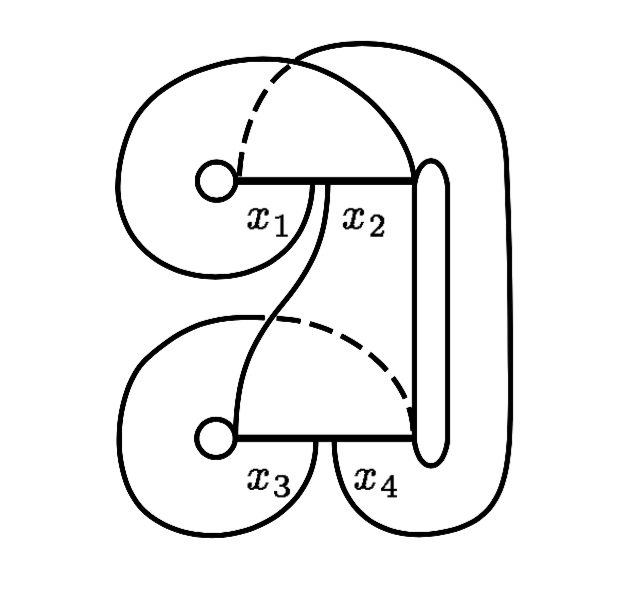
\includegraphics[width=0.5\textwidth]{universal}
  \caption{The universal template, reproduced from~\cite{knottyode}}\label{fig:universal}
\end{figure}



\subsection{Template renormalization}
Template renormalization exposition goes here. This should be done very carefully and in much greater detail than given in Ghrist, I think

\subsection{Braids}

\subsection{Link of knots}

\subsection{Renormalization}
\end{document}
